\documentclass[12pt]{report}
\usepackage[a4paper, margin=1in]{geometry}
\usepackage{graphicx}
\usepackage{setspace}
\usepackage{ragged2e}
\usepackage{fancyhdr}
\usepackage{url}
\usepackage[hidelinks,hypertexnames=false]{hyperref}
\usepackage{bookmark}
\usepackage{microtype}
\usepackage{tocloft}
\usepackage{float}

% Force dots for all entries in TOC
\renewcommand{\cftchapleader}{\cftdotfill{\cftdotsep}} 

\setlength{\headheight}{14.5pt}

% Customizing TOC, LOF, LOT Titles
\renewcommand{\contentsname}{CONTENTS}
\renewcommand{\listfigurename}{LIST OF FIGURES}
\renewcommand{\listtablename}{LIST OF TABLES}

\renewcommand{\cfttoctitlefont}{\hspace*{\fill}\Large\bfseries}
\renewcommand{\cftaftertoctitle}{\hspace*{\fill}}
\renewcommand{\cftloftitlefont}{\hspace*{\fill}\Large\bfseries}
\renewcommand{\cftafterloftitle}{\hspace*{\fill}}
\renewcommand{\cftlottitlefont}{\hspace*{\fill}\Large\bfseries}
\renewcommand{\cftafterlottitle}{\hspace*{\fill}}

\begin{document}
	
	% -------------------- ROMAN PAGE NUMBERING --------------------
	\pagenumbering{roman}
	
	% -------------------- HEADER / FOOTER --------------------
	\fancyhf{}
	\fancyhead[C]{\textbf{SecureVote Trust}}
	\fancyfoot[C]{\textbf{MCOERC}}
	\fancyfoot[R]{\thepage}
	\renewcommand{\headrulewidth}{0.4pt}
	\renewcommand{\footrulewidth}{0.4pt}
	\pagestyle{empty} % Disable headers/footers for front matter
	
	% -------------------- TITLE PAGE --------------------
	\begin{titlepage}
		\thispagestyle{empty}
		\centering
		\doublespacing
		
		{\Large \textbf{A Project Report on}}\\[1cm]
		
		{\LARGE \textbf{SecureVote Trust: Blockchain Voting with Face Authentication}}\\[1.5cm]
		
		\textbf{by}\\[0.5cm]
		
		\begin{tabular}{l}
			Dhanashri Sharad Pagar \\
			Srushti Prashant Sonawane \\
			Pranjal Mahesh Bhavsar \\
			Kirti Pravin Suryawanshi \\
		\end{tabular}\\[1.5cm]
		
		\textbf{Under the guidance of}\\[0.3cm]
		\textbf{Dr. S. A. Bhavsar}\\[1cm]
		
		
\includegraphics[width=0.3\textwidth]{logo_1.png}\\[1cm]
		
		\textbf{Department of Computer Engineering}\\
		Matoshri College of Engineering and Research Centre,\\
		Nashik-422105\\[0.2cm]
		
		\textbf{SAVITRIBAI PHULE PUNE UNIVERSITY}\\
		\textbf{Academic Year 2026--27}
		
	\end{titlepage}
	
	% -------------------- CERTIFICATE --------------------
	\newpage
	\thispagestyle{empty}
	
	\begin{center}
		\begin{singlespacing}
			\vspace*{0.2cm}
			{\Large \textbf{CERTIFICATE}}
			
			\vspace{0.6cm}
			{\small Matoshri Education Society's}
			
			\vspace{0.3cm}
			
\includegraphics[width=0.3\textwidth]{logo_1.png}
			
			\vspace{0.6cm}
			{\large \textbf{Department of Computer Engineering\\
					Matoshri College of Engineering and Research Centre, Nashik}}
		\end{singlespacing}
	\end{center}
	\addcontentsline{toc}{chapter}{Certificate}
	
	\vspace{1.5cm}
	\justifying
	\noindent This is to certify that \dotfill
	\noindent has successfully completed the project work on \textbf{``SecureVote Trust: Blockchain Voting with Face Authentication''} at Matoshri College of Engineering and Research Centre, Nashik in partial fulfillment of the Under Graduate course \textbf{B.E. (Computer Engineering)}, in academic year \textbf{2026--27} as prescribed by \textbf{Savitribai Phule Pune University}.
	
	\vspace{3cm}
	
	\noindent
	\begin{tabular*}{\textwidth}{@{\extracolsep{\fill}}ccc}
		\textbf{Dr. S. A. Bhavsar} & \textbf{Dr. S. A. Bhavsar} & \textbf{Dr. G. K. Kharate} \\
		Project Guide & Head of Department & Principal
	\end{tabular*}
	
	\vspace{2cm}
	\begin{flushleft}
		\textbf{Examiner Name and Sign}\\
		\textbf{Date:} 
	\end{flushleft}
	
	\newpage
	
	% -------------------- ACKNOWLEDGEMENT --------------------
	\begin{center}
		{\Large \textbf{ACKNOWLEDGEMENT}}
	\end{center}
	\addcontentsline{toc}{chapter}{Acknowledgement}
	
	\doublespacing
	
	First and foremost, I express my deep sense of gratitude, sincere thanks, and appreciation to my project guide \textbf{Dr. S. A. Bhavsar} and Project coordinator \textbf{Ms. S. A. Handore}, Department of Computer Engineering, Matoshri College of Engineering and Research Centre, Nashik. Your availability at any time throughout the semester, valuable guidance, comments, constructive criticism, encouragement, and support tremendously boosted this research work.
	
	Again, loads and loads of thanks to the Head of Computer Engineering Department, \textbf{Dr. S. A. Bhavsar}, for providing me with constant support and motivation. Your opinions, views, and thoughts have truly helped me improve my work and writing.
	
	I would also like to express my sincere gratitude to \textbf{Dr. G. K. Kharate}, Principal, Matoshri College of Engineering and Research Centre, Nashik, for providing a great platform to complete this work within the scheduled time.
	
	I am also thankful to all the faculty members of the Department of Computer Engineering, Matoshri College of Engineering and Research Centre, Nashik, for their valuable comments, encouragement, and help during the completion of this project.
	
	Last but not least, I would like to thank my family and friends from the bottom of my heart for their never-ending love, help, and support in so many ways throughout this time. Thank you so much.
	
	Finally, I thank the Almighty God for giving me the courage and confidence to complete not only this dissertation work but also to face every difficult situation in life.
	
	\newpage
	
	% -------------------- ABSTRACT --------------------
	\begin{center}
		{\Large \textbf{ABSTRACT}}
	\end{center}
	\addcontentsline{toc}{chapter}{Abstract}
	
	\doublespacing
	
	Electronic voting systems offer an alternative to traditional paper-based elections by improving voting efficiency, accessibility, and result processing. However, ensuring secure voter authentication, vote integrity, ballot privacy, and election transparency remains a major challenge. Blockchain technology provides tamper-evident and auditable transaction records, while facial recognition offers a biometric approach to verifying voter identity. Integrating these technologies may strengthen electronic voting security, but it also introduces challenges related to biometric privacy, spoofing attacks, scalability, and secure ballot management.
	
	This review paper examines existing research on blockchain-based electronic voting systems integrated with facial authentication and related biometric technologies. It discusses the fundamentals of blockchain, facial recognition, liveness detection, cryptographic protection, and ballot privacy. Existing research approaches are compared based on their authentication mechanisms, blockchain architectures, security features, privacy protections, and implementation challenges. The review further identifies research gaps concerning reliable biometric verification, voter anonymity, prevention of duplicate voting, secure vote recording, and system scalability. Finally, potential research directions are discussed for developing electronic voting systems that provide stronger security, privacy, transparency, accessibility, and verifiability. The study highlights the importance of combining appropriate technological safeguards with rigorous security evaluation and responsible system design before practical deployment.
	
	\vspace{0.5cm}
	\noindent
	\textbf{Keywords:} Blockchain Technology, Electronic Voting, Face Authentication, Biometric Verification, Liveness Detection, Ballot Privacy, Cryptographic Security, Election Integrity.
	
	
	\newpage
	
	% -------------------- AUTOMATIC INDEXING --------------------
	\tableofcontents
	\newpage
	
	\addcontentsline{toc}{chapter}{\listfigurename}
	\listoffigures
	\newpage
	
	\addcontentsline{toc}{chapter}{\listtablename}
	\listoftables
	\newpage
	
	% -------------------- SWITCH TO ARABIC --------------------
	\pagenumbering{arabic}
	\setcounter{page}{1}
	\pagestyle{fancy} % Enable headers/footers for main content
	
	% -------------------- CHAPTER 1 --------------------
	\chapter{Introduction}
	
	\section{Introduction}
	Electronic voting (e-voting) is an emerging approach to conducting elections using electronic devices and computer-based systems instead of relying entirely on traditional paper-based procedures. It offers several potential advantages, including faster vote counting, reduced manual effort, improved accessibility, and efficient election result management. However, ensuring the security, accuracy, transparency, and reliability of electronic voting systems remains a major concern.
	
	Traditional electronic voting systems may depend on centralized databases and conventional authentication mechanisms. Such systems can face security risks, including unauthorized access, data manipulation, identity theft, and technical failures. Furthermore, maintaining voter privacy and preventing duplicate voting are important requirements for establishing public trust in electronic elections. These challenges have encouraged researchers to explore advanced technologies for improving voting system security.
	
	Blockchain technology has gained attention as a potential solution for maintaining secure and verifiable electronic voting records. It uses cryptographic hashing and linked data blocks to create a tamper-evident transaction history. Depending on its implementation, blockchain can improve transaction traceability, support independent auditing, and make unauthorized modifications easier to detect. However, blockchain alone cannot guarantee voter anonymity, ballot secrecy, or the correctness of recorded votes.
	
	Biometric authentication provides another approach to improving voter identity verification. Facial recognition technology identifies individuals by analyzing facial features captured through a camera. It can be integrated into electronic voting systems to verify registered voters before allowing access to the voting process. Additionally, liveness detection techniques can help distinguish a live person from certain presentation attacks, such as photographs or displayed facial images.
	
	Combining blockchain technology with facial authentication creates an opportunity to develop more secure and transparent electronic voting architectures. Facial authentication can support voter verification, while blockchain can maintain auditable voting transactions. Cryptographic techniques, including encryption, digital signatures, and zero-knowledge proofs, can further support data protection and verification. Nevertheless, the integration must carefully protect biometric information and ensure that voter identities cannot be linked to their ballot choices.
	
	This review paper examines existing research on blockchain-based electronic voting systems integrated with facial authentication and related security technologies. It analyzes different approaches, compares their features, identifies security and privacy challenges, and highlights research gaps that require further investigation.
	
	\section{Objectives}
	The main objectives of this review paper are:
	\begin{enumerate}
		\item To study existing blockchain-based electronic voting systems and understand their architectures, working principles, and security mechanisms.
		\item To examine facial recognition and biometric authentication techniques used for voter identity verification.
		\item To analyze the role of liveness detection in reducing facial presentation attacks and unauthorized authentication.
		\item To compare existing research approaches based on vote integrity, voter privacy, authentication, scalability, and transaction verification.
		\item To identify research gaps and explore future directions for developing secure, transparent, privacy-preserving, and reliable electronic voting systems.
	\end{enumerate}
	
	\section{Scope of the Review}
	This review focuses on academic research related to blockchain-based electronic voting, facial authentication, biometric verification, cryptographic protection, and ballot privacy. It considers different blockchain architectures, authentication approaches, and security mechanisms proposed in existing studies. The review also examines challenges associated with biometric data protection, voter anonymity, duplicate voting prevention, system performance, and election verifiability.
	
	\section{Organization of the Review Paper}
	The remainder of this paper is organized as follows: Chapter 2 discusses the background and related technologies. Chapter 3 presents the literature review and comparative analysis of existing research. Chapter 4 examines security, privacy challenges, and identified research gaps. Chapter 5 discusses future research directions, and the final chapter presents the conclusion and references.
	
	% -------------------- CHAPTER 2 --------------------
	
	\chapter{Literature Survey}
	
	\section{Introduction}
	Electronic voting security has become an important research area due to concerns regarding voter authentication, vote integrity, ballot privacy, and election transparency. Researchers have explored blockchain technology, biometric authentication, Internet of Things (IoT), and advanced cryptographic techniques to address these challenges. This chapter reviews selected research publications and compares their proposed approaches, technologies, contributions, and implementation considerations.
	
	\section{Review of Existing Research}
	
	\noindent\textbf{1. Ajao et al. (2025)}\\
	Ajao et al. proposed a blockchain-integrated electronic voting system using multimodal biometric authentication. The approach combines facial and fingerprint recognition for voter identity verification and blockchain technology for maintaining verifiable voting records. It also incorporates homomorphic encryption to protect sensitive voting information. The study demonstrates the potential of combining multiple biometric modalities with blockchain. However, integrating multiple biometric techniques may increase computational requirements and implementation complexity. Biometric data protection and voter anonymity also require careful consideration.
	
	\vspace{0.3cm}
	\noindent\textbf{2. Rifat et al. (2026)}\\
	Rifat et al. presented a blockchain-integrated IoT biometric architecture for secure and decentralized electronic voting. Their research explores the integration of biometric authentication, IoT devices, and blockchain technology to strengthen voter verification and voting transaction management. The approach highlights the potential of connected biometric infrastructure in electronic elections. However, practical implementation requires attention to IoT device security, network reliability, biometric information protection, and system scalability.
	
	\vspace{0.3cm}
	\noindent\textbf{3. Alsuwat (2026)}\\
	Alsuwat proposed a secure electronic voting framework combining blockchain, Dilithium digital signatures, and zero-knowledge proof verification. Dilithium provides post-quantum digital signature authentication, while zero-knowledge proofs enable verification of voter eligibility and ballot conditions without revealing sensitive information. The framework also incorporates encrypted ballots, nullifier-based double-voting prevention, smart contracts, and Byzantine fault-tolerant consensus in a permissioned blockchain network. Its experimental evaluation reported a throughput of 408 transactions per second and an average block finalization time of 2.18 seconds. However, cryptographic proof generation and verification introduce computational overhead that requires consideration during large-scale deployment.
	
	\section{Summary of Literature Survey}
	The reviewed studies demonstrate different approaches to improving electronic voting security. Ajao et al. focus on multimodal biometric authentication, Rifat et al. explore IoT-based biometric voting infrastructure, and Alsuwat investigates post-quantum authentication and privacy-preserving cryptographic verification.
	
	The comparison indicates that blockchain can support transaction integrity and auditing, biometric authentication can assist voter identity verification, and advanced cryptographic techniques can strengthen authentication and privacy. However, challenges remain in protecting biometric information, maintaining ballot secrecy, preventing duplicate voting, ensuring scalability, and providing reliable election verification. These findings highlight the need for an integrated voting architecture that balances security, privacy, performance, and usability.
	
	\newpage
	\section{Literature Survey Comparison Table}
	
	\begin{table}[h!]
		\centering
		\small
		\renewcommand{\arraystretch}{1.6}
		\caption{Literature Survey Comparison Table}
		\vspace{0.2cm}
		\label{tab:lit_survey}
		\begin{tabular}{|p{3.2cm}|p{3.8cm}|p{3.8cm}|p{4.2cm}|}
			\hline
			\textbf{Parameter} & \textbf{Ajao et al. (2025)} & \textbf{Rifat et al. (2026)} & \textbf{Alsuwat (2026)} \\ \hline
			Research focus & Multimodal biometric blockchain voting & IoT biometric voting & Privacy-preserving blockchain voting \\ \hline
			Technologies & Blockchain, face and fingerprint recognition & Blockchain, IoT, biometrics & Blockchain, Dilithium, zero-knowledge proofs \\ \hline
			Authentication & Multimodal biometrics & Biometric authentication & Post-quantum digital signatures \\ \hline
			Privacy mechanism & Homomorphic encryption & Not specified here & Zero-knowledge proofs and encrypted ballots \\ \hline
			Double-voting prevention & Not specified here & Not specified here & Nullifier-based prevention \\ \hline
			Blockchain architecture & Blockchain-based voting & Decentralized IoT biometric architecture & Permissioned blockchain \\ \hline
			Consensus mechanism & Not specified here & Not specified here & Byzantine fault-tolerant consensus \\ \hline
			Reported performance & Refer to original paper & Refer to original paper & 408 TPS; 2.18-second average block finalization \\ \hline
			Key consideration & Biometric integration complexity & IoT security and scalability & Cryptographic computational overhead \\ \hline
		\end{tabular}
	\end{table}
	
	\newpage
	
	% -------------------- CHAPTER 3 --------------------
	\chapter{Software Requirement Specification}
	
	\section{Introduction}
	The Software Requirement Specification (SRS) defines the functional and non-functional requirements of the proposed Blockchain Voting with Face Authentication system. The system aims to provide a secure, transparent, and reliable electronic voting platform. It combines facial recognition, liveness detection, cryptographic techniques, and blockchain technology to authenticate voters and maintain tamper-evident voting records.
	
	\section{System Features}
	The proposed system includes the following features:
	\begin{enumerate}
		\item \textbf{Voter Registration:} Allows voters to register by submitting their personal information and facial data for verification.
		\item \textbf{Admin Management:} Enables administrators to approve voters, manage elections, add candidates, and monitor voting activities.
		\item \textbf{Face Authentication:} Uses facial recognition to verify the identity of registered voters before allowing access to the voting system.
		\item \textbf{Liveness Detection:} Uses MediaPipe-based verification to help detect attempts involving photographs or prerecorded facial videos.
		\item \textbf{Secure Voting:} Allows authenticated voters to select candidates and submit their votes securely.
		\item \textbf{Blockchain Integration:} Records vote-related transactions in a local blockchain structure to support integrity verification and auditing.
		\item \textbf{Duplicate Voting Prevention:} Ensures that an eligible voter cannot submit more than one vote in the same election.
		\item \textbf{Result Management:} Provides election results and voting statistics after the election process is completed.
	\end{enumerate}
	
	\section{Hardware and Software Requirements}
	
	\subsection{Hardware Requirements}
	The following hardware specifications are proposed for development and testing:
	
	\begin{table}[h!]
		\centering
		\renewcommand{\arraystretch}{1.6}
		\renewcommand{\arraystretch}{1.6}
		\caption{Hardware Requirements}
		\vspace{0.2cm}
		\label{tab:hardware_req}
		\begin{tabular}{|p{5cm}|p{9.5cm}|}
			\hline
			\textbf{Component} & \textbf{Minimum Requirement} \\ \hline
			Processor & Intel Core i5 / equivalent \\ \hline
			RAM & 8 GB \\ \hline
			Storage & 256 GB SSD \\ \hline
			Camera & 720p webcam \\ \hline
			Display & 1366 $\times$ 768 resolution \\ \hline
			Network & Internet or local network connection \\ \hline
		\end{tabular}
	\end{table}
	\newpage
	\subsection{Software Requirements}
	\begin{table}[h!]
		\centering
		\renewcommand{\arraystretch}{1.6}
		\renewcommand{\arraystretch}{1.6}
		\caption{Software Requirements}
		\vspace{0.2cm}
		\label{tab:software_req}
		\begin{tabular}{|p{5cm}|p{9.5cm}|}
			\hline
			\textbf{Software} & \textbf{Technology} \\ \hline
			Operating System & Windows 10/11 \\ \hline
			Frontend & React.js, HTML, CSS, JavaScript \\ \hline
			Backend & Python, FastAPI \\ \hline
			Database & SQLite \\ \hline
			Face Recognition & OpenCV \\ \hline
			Liveness Detection & MediaPipe \\ \hline
			Authentication & JWT \\ \hline
			Cryptography & AES, RSA, SHA-256, Digital Signatures \\ \hline
			Blockchain & Local Python-based blockchain \\ \hline
			Development Tools & VS Code, Web Browser \\ \hline
		\end{tabular}
	\end{table}
	
	\newpage
	\section{Functional Requirements}
	\begin{itemize}
		\item The system shall allow administrators to manage voters, candidates, and elections.
		\item The system shall allow voters to register and submit facial information.
		\item The system shall authenticate voters using facial recognition and liveness detection.
		\item The system shall allow only approved and authenticated voters to access active elections.
		\item The system shall prevent duplicate voting within an election.
		\item The system shall securely process votes and record corresponding blockchain transactions.
		\item The system shall provide transaction verification, audit logs, and election results.
	\end{itemize}
	
	\section{Non-Functional Requirements}
	\begin{itemize}
		\item \textbf{Security:} Protect user credentials and sensitive information using authentication and encryption.
		\item \textbf{Reliability:} Maintain consistent voting operations and transaction records.
		\item \textbf{Performance:} Provide timely facial verification and vote processing.
		\item \textbf{Scalability:} Support an increasing number of voters and election records.
		\item \textbf{Usability:} Provide a simple and accessible interface for administrators and voters.
		\item \textbf{Integrity:} Maintain tamper-evident voting records through blockchain hashing and verification.
	\end{itemize}
	
	\section{Project Timeline Chart}
	The proposed development schedule is planned over eight weeks, followed by final review and submission.
	
	\begin{table}[h!]
		\centering
		\renewcommand{\arraystretch}{1.65}
		\renewcommand{\arraystretch}{1.65}
		\caption{Project Timeline Chart}
		\vspace{0.2cm}
		\label{tab:timeline}
		\begin{tabular}{|p{4.5cm}|p{2.8cm}|p{8.2cm}|}
			\hline
			\textbf{Phase} & \textbf{Duration} & \textbf{Activities} \\ \hline
			Requirement Analysis & Week 1 & Identify requirements and finalize SRS \\ \hline
			System Design & Week 2 & Architecture, database, and UI design \\ \hline
			Frontend Development & Week 3 & React interface and user modules \\ \hline
			Backend Development & Week 4 & FastAPI and SQLite integration \\ \hline
			Face Authentication & Week 5 & Facial recognition and liveness detection \\ \hline
			Blockchain Integration & Week 6 & Secure transactions and verification \\ \hline
			Testing and Debugging & Week 7 & Functional, security, and integration testing \\ \hline
			Finalization & Week 8 & Documentation and final corrections \\ \hline
			Final Review & 1 January 2027 & Project review and submission \\ \hline
		\end{tabular}
	\end{table}
	
	\vspace{0.5cm}
	\noindent The proposed SRS establishes the technical foundation for developing the voting application. The combination of biometric authentication, cryptographic protection, and blockchain-based record verification is intended to improve voter verification and voting-record integrity. The system is designed as a local blockchain prototype for academic implementation and testing.
	
	% -------------------- CHAPTER 4 --------------------
	\chapter{System Design}
	
	\section{System Architecture}
	
	\begin{figure}[H]
		\centering
		\fbox{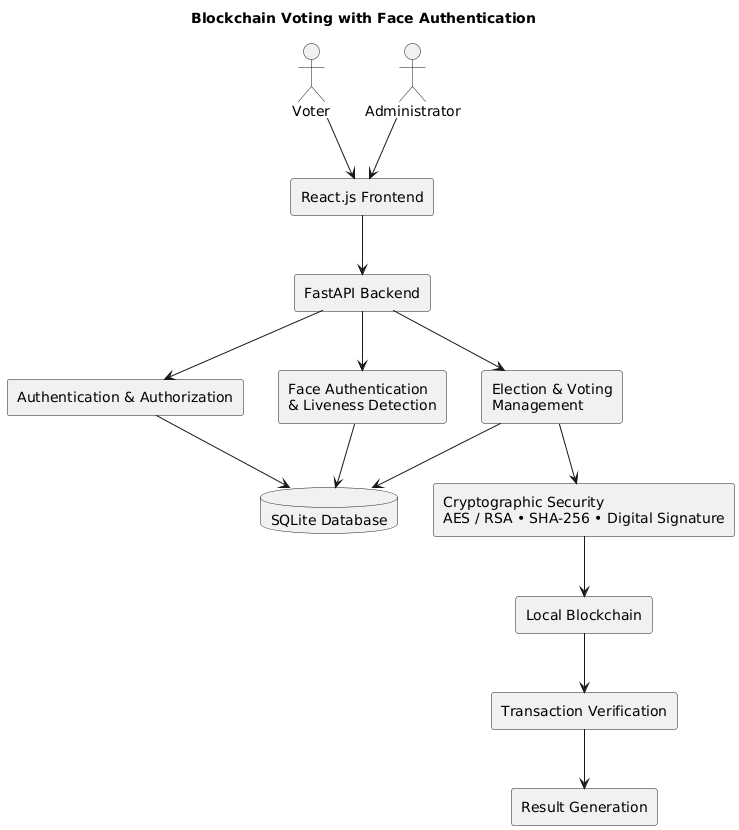
\includegraphics[width=0.9\textwidth, height=11.5cm, keepaspectratio]{system_architecture.png}} 
		\caption{System Architecture of Blockchain Voting with Face Authentication}
		\label{fig:sys_arch}
	\end{figure}
	
	The system architecture describes the overall structure of the proposed Blockchain Voting with Face Authentication system. It consists of multiple layers that work together to provide secure voter registration, identity verification, election management, and vote recording.
	
	The presentation layer is developed using React.js and provides separate interfaces for administrators and voters. The application layer uses FastAPI to handle user requests, authentication, election operations, and voting processes. The biometric verification layer uses OpenCV for facial recognition and MediaPipe for liveness detection. The security layer applies encryption, hashing, and digital signatures to protect sensitive information. The data storage layer uses SQLite for application records and a local Python-based blockchain for maintaining tamper-evident voting transactions.
	
	\newpage
	\section{Data Flow Diagrams}
	Data Flow Diagrams (DFDs) represent how information moves between users, system processes, and data storage components. They help understand the interaction between external entities and internal system operations.
	
	\subsection{DFD Level 0 Diagram}
	
	\begin{figure}[H]
		\centering
		\fbox{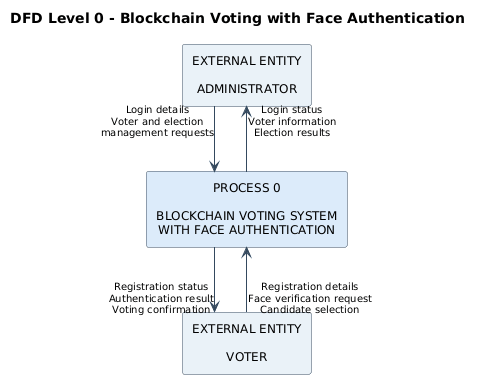
\includegraphics[width=0.9\textwidth, height=10.5cm, keepaspectratio]{dfdl0.png}}
		\caption{DFD Level 0 -- Context Diagram}
		\label{fig:dfd0}
	\end{figure}
	
	The Level 0 DFD, also called the Context Diagram, represents the entire voting application as a single process. It shows two main external entities: Administrator and Voter. The administrator provides login details and election management information, while the voter submits registration details, facial information, and voting requests. The system returns authentication status, registration information, voting confirmation, and election results.
	
	\newpage
	\subsection{DFD Level 1 Diagram}
	
	\begin{figure}[H]
		\centering
		\fbox{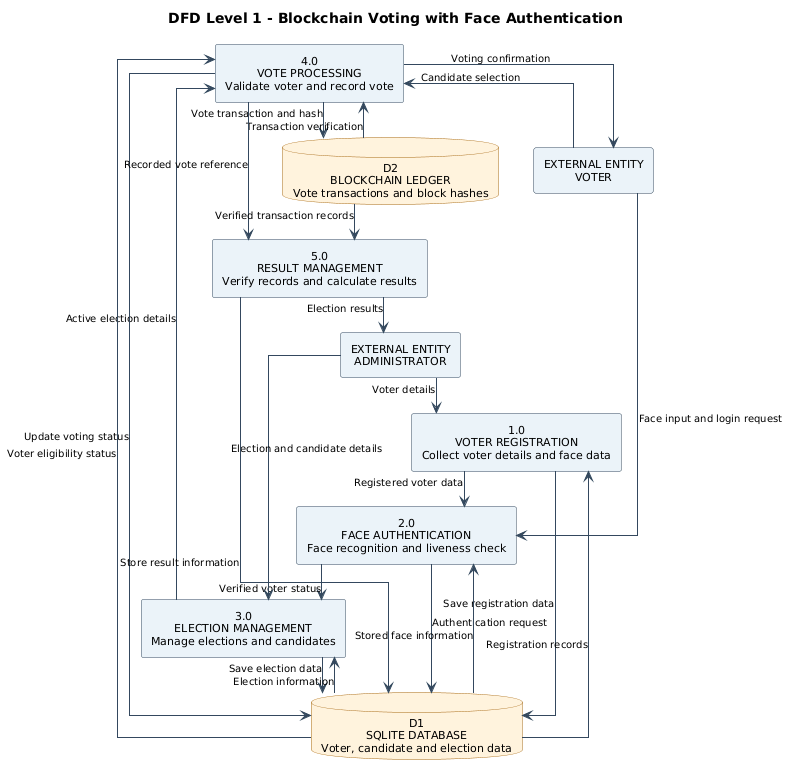
\includegraphics[width=0.95\textwidth, height=22cm, keepaspectratio]{dfdl1.png}} 
		\caption{DFD Level 1 -- Detailed Data Flow Diagram}
		\label{fig:dfd1}
	\end{figure}
	
	The Level 1 DFD expands the main system into smaller processes, including voter registration, face authentication, election management, vote processing, and result management. It also represents the SQLite database and blockchain ledger. Information is exchanged between these processes to verify voter eligibility, manage elections, process votes, and maintain transaction records.
	
	\newpage
	\section{UML Diagrams}
	Unified Modeling Language (UML) diagrams describe the structure, behaviour, and interactions of the proposed system. They provide a visual representation of the system's functional requirements and internal design.
	
	\subsection{Use Case Diagram}
	
	\begin{figure}[H]
		\centering
		\fbox{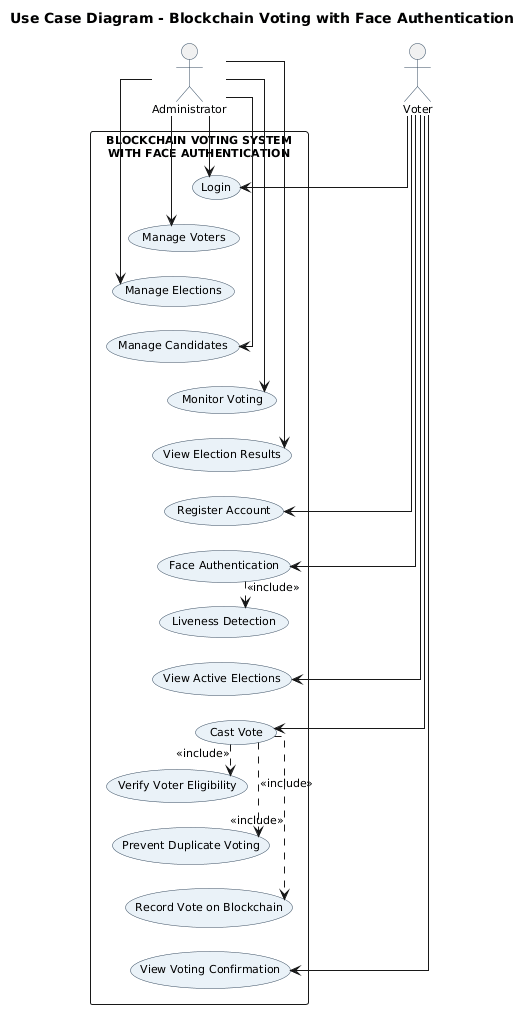
\includegraphics[width=5.85\textwidth, height=16.5cm, keepaspectratio]{use case.png}} 
		\caption{UML Use Case Diagram}
		\label{fig:usecase}
	\end{figure}
	
	The Use Case Diagram represents the interactions between the Administrator and Voter. The administrator manages voters, elections, candidates, and results. The voter registers, completes face authentication, views active elections, and casts a vote. It also shows supporting activities such as liveness detection and duplicate-voting prevention.
	
	\subsection{Sequence Diagram}
	
	\begin{figure}[H]
		\centering
		\fbox{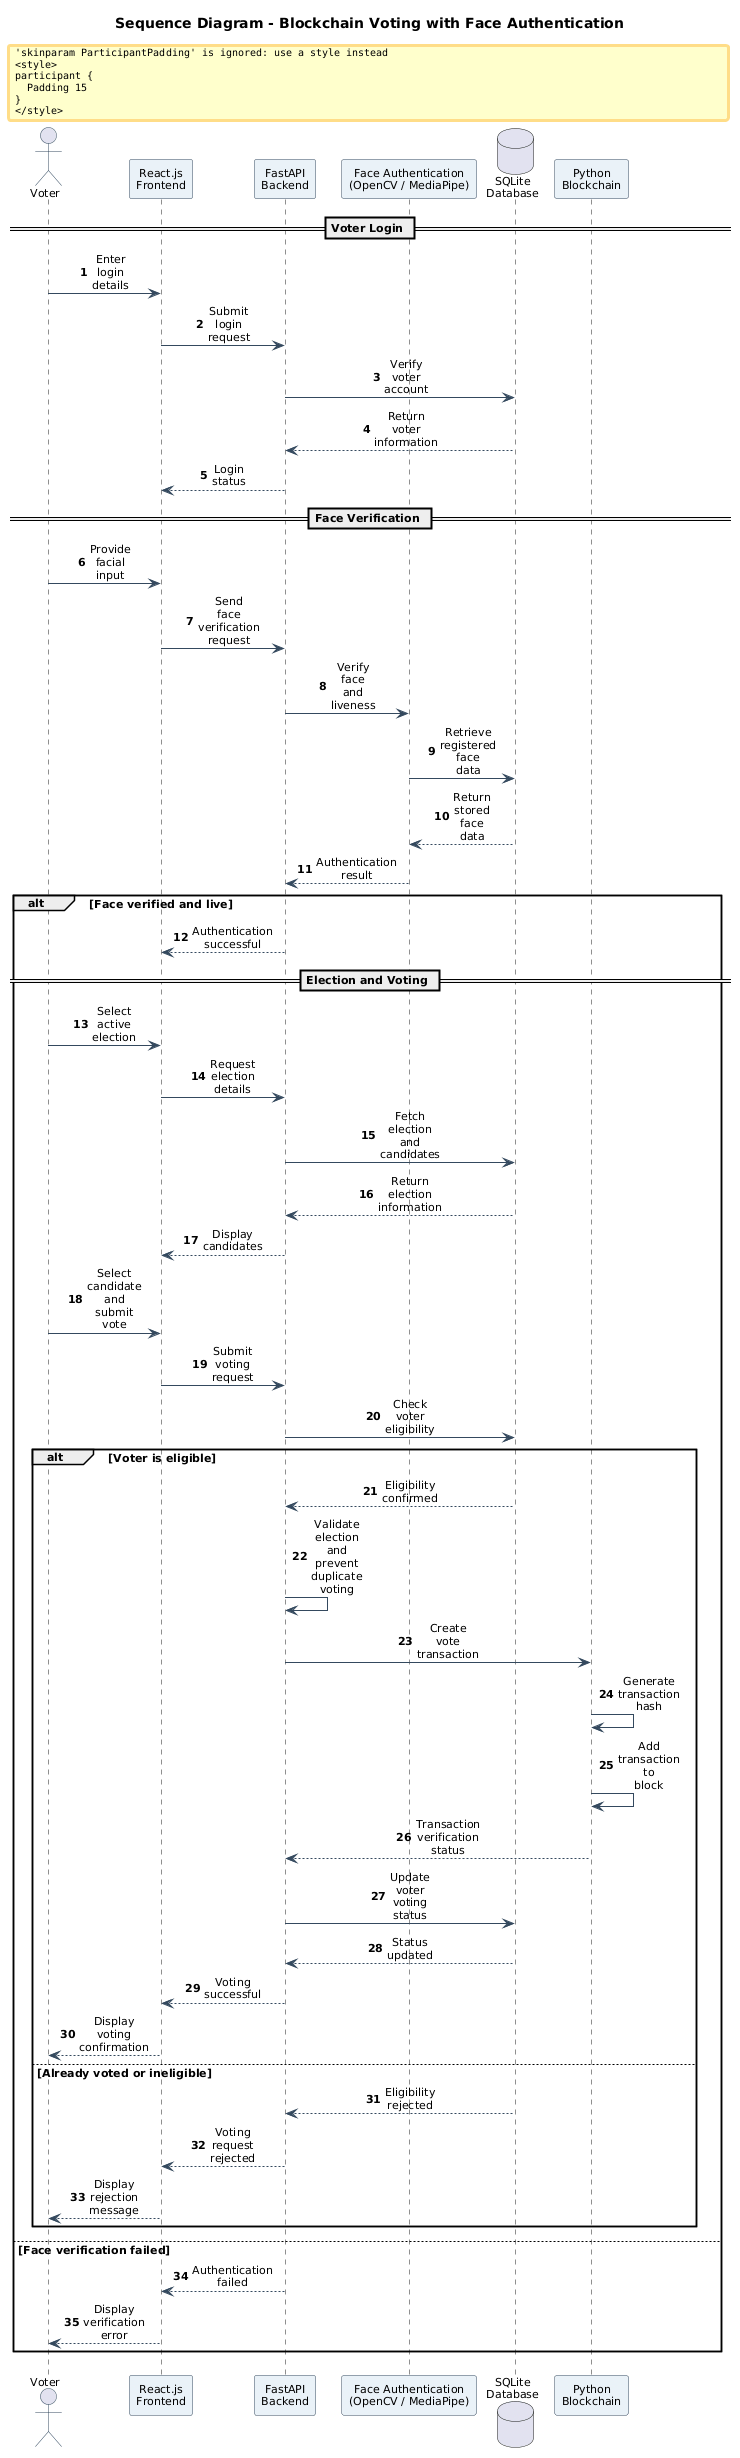
\includegraphics[width=\textwidth, height=17cm, keepaspectratio]{SequenceDiagram.png}} 
		\caption{UML Sequence Diagram}
		\label{fig:sequence}
	\end{figure}
	
	The Sequence Diagram illustrates the chronological flow of communication between the voter, React frontend, FastAPI backend, face authentication module, SQLite database, and blockchain. It explains the login process, biometric verification, election selection, vote validation, transaction creation, and voting confirmation.
	\subsection{Class Diagram}
	
	\begin{figure}[H]
		\centering
		\fbox{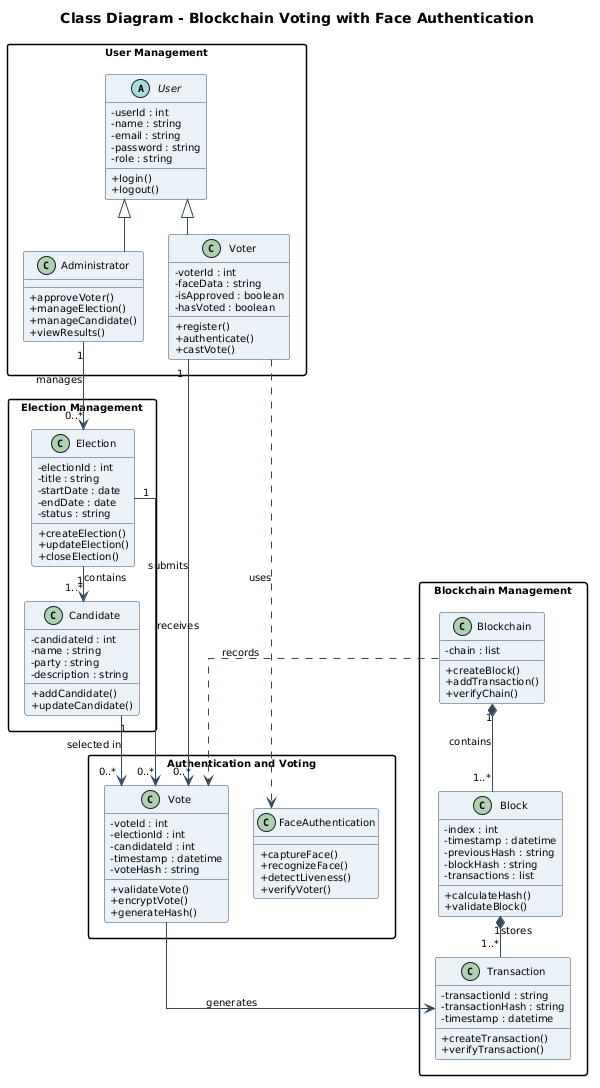
\includegraphics[width=0.95\textwidth, height=14cm, keepaspectratio]{class diagram.png}} 
		\caption{UML Class Diagram}
		\label{fig:class}
	\end{figure}
	
	The Class Diagram represents the static structure of the application. It includes classes such as User, Administrator, Voter, Election, Candidate, FaceAuthentication, Vote, Blockchain, Block, and Transaction. It describes their attributes, methods, inheritance, and relationships, providing a logical view of the application's object-oriented design.
	
	\newpage
	\subsection{Activity Diagram}
	
	\begin{figure}[H]
		\centering
		\fbox{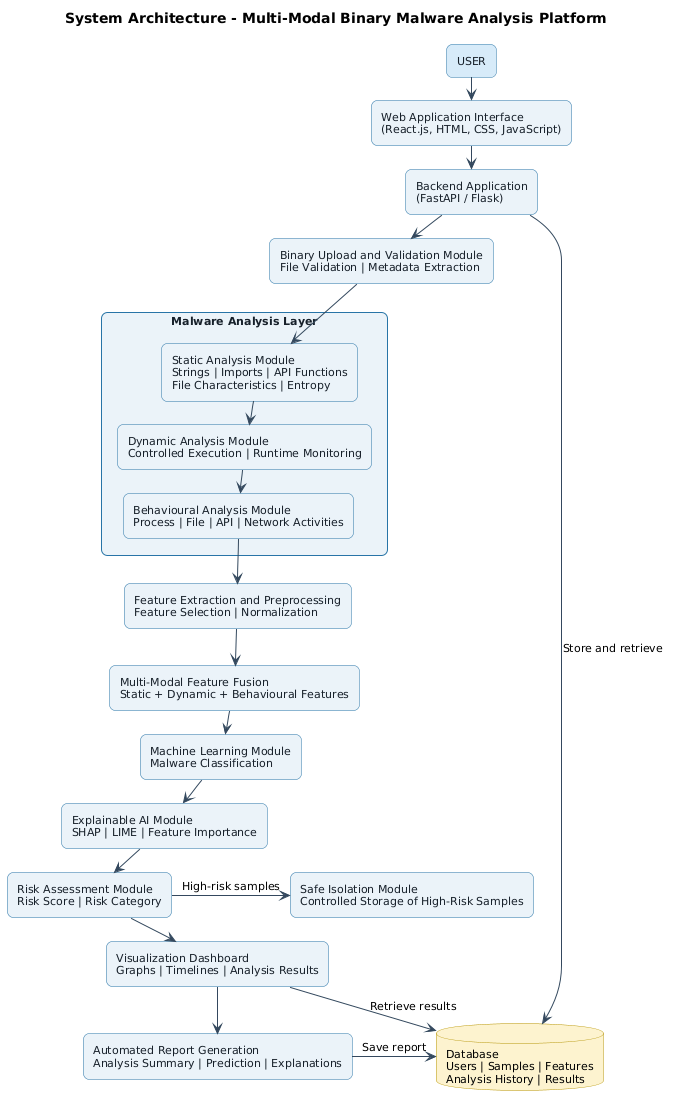
\includegraphics[width=0.85\textwidth, height=17cm, keepaspectratio]{Activity Diagram.png}} 
		\caption{UML Activity Diagram}
		\label{fig:activity}
	\end{figure}
	
	The Activity Diagram describes the complete workflow of the voting application. It starts with voter registration and administrator approval, followed by login, face recognition, and liveness detection. After successful authentication, the voter selects an election and candidate. The system checks eligibility, processes the vote, generates a transaction hash, and verifies the blockchain transaction before displaying confirmation.
	
	\newpage
	\subsection{User Activity Diagram}
	
	\begin{figure}[H]
		\centering
		\fbox{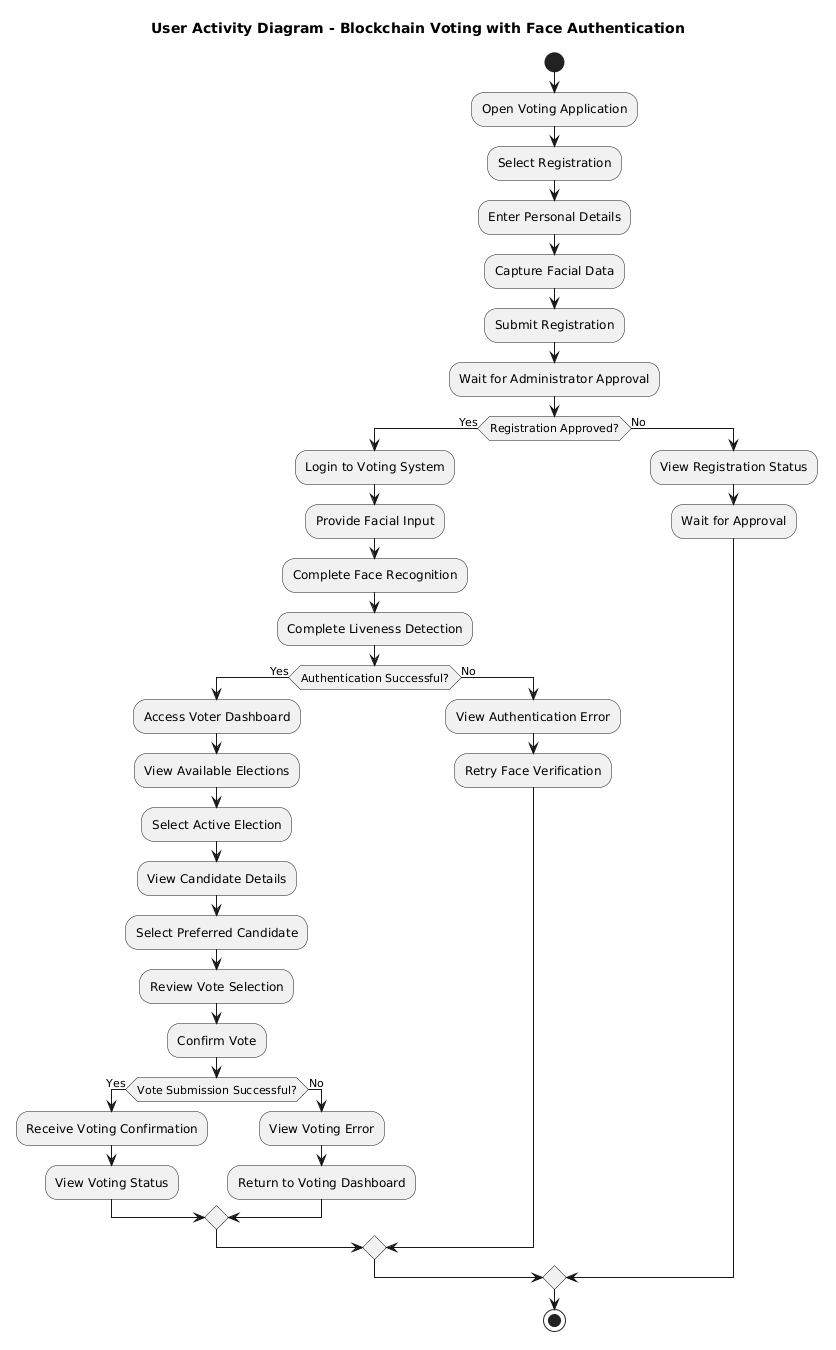
\includegraphics[width=0.85\textwidth, height=11.5cm, keepaspectratio]{user activity.png}} 
		\caption{User Activity Diagram}
		\label{fig:useractivity}
	\end{figure}
	
	The User Activity Diagram focuses specifically on the activities performed by the voter. It illustrates the user's journey from registration and approval to login, facial verification, election selection, candidate selection, vote confirmation, and viewing the final voting status. It also represents alternative paths when registration or authentication fails.
	
	The User Activity Diagram focuses specifically on the activities performed by the voter. It illustrates the user's journey from registration and approval to login, facial verification, election selection, candidate selection, vote confirmation, and viewing the final voting status. It also represents alternative paths when registration or authentication fails.
	
	\section{Summary}
	The system design provides a structured representation of the proposed voting application. The architecture defines the major technical components, DFDs explain information flow, and UML diagrams describe system interactions and behaviour. Together, these diagrams establish the foundation for the implementation and testing phases.
	
		% -------------------- CHAPTER 5 --------------------
	\newpage
	\chapter{Expected Results and Discussion}
	
	\section{Expected Results}
	The proposed Blockchain Voting with Face Authentication system is expected to provide a secure, transparent, and user-friendly electronic voting platform. By integrating facial recognition, liveness detection, cryptographic techniques, and blockchain technology, the system aims to improve voter verification and voting-record integrity.
	
	The expected results of the project are as follows:
	\begin{enumerate}
		\item \textbf{Secure Voter Registration:} The system is expected to allow voters to register by submitting personal information and facial data. Administrators will be able to review and approve voter registrations.
		\item \textbf{Accurate Face Authentication:} OpenCV-based facial recognition is expected to identify registered voters by comparing captured facial information with stored reference data.
		\item \textbf{Liveness Detection:} MediaPipe-based liveness detection is expected to help identify presentation attacks involving photographs or prerecorded videos, reducing unauthorized access attempts.
		\item \textbf{Duplicate Voting Prevention:} The system is expected to restrict each approved voter to one vote per election through eligibility checks and voting-status management.
		\item \textbf{Blockchain-Based Record Integrity:} Voting transactions are expected to be recorded in a local Python-based blockchain. Hash generation and verification will help detect unauthorized modifications to recorded transactions.
		\item \textbf{Secure Data Management:} Encryption, hashing, and digital signatures are expected to provide additional protection for sensitive information and voting transactions.
		\item \textbf{Election Result Management:} The system is expected to generate election results and voting statistics based on successfully recorded votes.
	\end{enumerate}
	
	\section{Discussion}
	The proposed system combines biometric authentication and blockchain technology to address important limitations of conventional electronic voting approaches. Facial recognition provides an additional method of verifying voter identity, while liveness detection helps reduce the risk of identity spoofing. Blockchain technology provides a tamper-evident structure for maintaining voting transactions and supporting auditability.
	
	The integration of React.js and FastAPI is expected to provide a responsive user interface and efficient backend communication. SQLite will manage application information, while the local blockchain will maintain transaction records.
	
	However, the system may face challenges related to facial recognition accuracy under different lighting conditions, camera quality, network availability, processing time, and computational requirements. Biometric information must be securely stored, and voter identity must remain separate from ballot selections to protect voting privacy. The local blockchain implementation also has limitations compared with a distributed production blockchain network.
	
	\section{Overall Outcome}
	The expected outcome is a functional prototype that demonstrates voter registration, face authentication, liveness detection, secure vote processing, duplicate-voting prevention, blockchain transaction verification, and election result generation. The project will demonstrate how biometric verification and blockchain-based record management can be integrated into an electronic voting application.

			% -------------------- CHAPTER 6 --------------------
	\chapter{Conclusions and Future Scope}
	
	\section{Conclusion}
	The proposed project, \textbf{Blockchain Voting with Face Authentication}, aims to develop a secure, transparent, and reliable electronic voting system by integrating blockchain technology with biometric authentication. The system combines facial recognition, liveness detection, cryptographic techniques, and blockchain-based transaction management to improve voter verification and voting-record integrity.
	
	The proposed application uses React.js for the frontend, FastAPI for backend services, and SQLite for database management. OpenCV and MediaPipe are used for facial recognition and liveness detection, respectively. Cryptographic techniques such as encryption, hashing, and digital signatures provide additional security, while the local Python-based blockchain maintains tamper-evident voting transactions.
	
	The system is designed to support voter registration, administrator approval, face authentication, election management, candidate selection, duplicate-voting prevention, transaction verification, and election result generation.
	
	Overall, the project demonstrates the potential of combining biometric authentication and blockchain technology in electronic voting applications. Although the proposed system is an academic prototype, it provides a foundation for further research and development in secure digital election management. Additional testing, privacy controls, and scalability improvements will be necessary before considering real-world election deployment.
	
	\section{Future Scope}
	The proposed system can be enhanced in several ways to improve its security, performance, scalability, and practical usability.
	
	\begin{enumerate}
		\item \textbf{Distributed Blockchain Integration:} The local Python blockchain can be extended to a distributed blockchain network with multiple authorized nodes to improve decentralization and independent transaction verification.
		\item \textbf{Advanced Biometric Authentication:} Future versions can integrate multimodal biometrics, such as facial recognition and fingerprint verification, to provide additional identity verification capabilities.
		\item \textbf{Enhanced Privacy Protection:} Advanced cryptographic techniques, including zero-knowledge proofs and homomorphic encryption, can be explored to strengthen ballot privacy while supporting independent verification.
		\item \textbf{Cloud-Based Deployment:} The application can be deployed on secure cloud infrastructure to support larger numbers of voters, improved availability, and centralized system monitoring.
		\item \textbf{Performance and Security Testing:} Further work can include large-scale load testing, penetration testing, biometric accuracy evaluation, and vulnerability assessment to identify and address system limitations.
	\end{enumerate}
	
	\vspace{0.3cm}
	\noindent These enhancements can help develop the proposed academic prototype into a more scalable, secure, privacy-preserving, and reliable electronic voting platform.
	
	\newpage
	\chapter*{References}
	\addcontentsline{toc}{chapter}{References}
	
	\begin{enumerate}
		\item J. Brownlee, \textit{Deep Learning for Natural Language Processing}, Machine Learning Mastery, 2019.
		
		\item D. Jurafsky and J. H. Martin, \textit{Speech and Language Processing}, 3rd Edition (Draft), Pearson Education, 2023.
		
		\item S. Poria, E. Cambria, R. Bajpai, and A. Hussain, “A review of affective computing: From unimodal analysis to multimodal fusion,” Information Fusion, vol. 37, pp. 98–125, 2017.
		
		\item A. Pandey and S. D. Kumar, “Speech Emotion Recognition using Deep Learning Techniques,” IEEE Access, vol. 9, pp. 94725–94735, 2021.
		
		\item M. Chen, X. Xu, and S. Zhang, “Automatic Interview Evaluation System Based on Artificial Intelligence,” International Journal of Advanced Computer Science and Applications (IJACSA), vol. 12, no. 9, 2021.
		
		\item M. Valstar et al., “AVEC 2016: Depression, Mood, and Emotion Recognition Workshop and Challenge,” Proceedings of the 6th International Workshop on Audio/Visual Emotion Challenge, 2016.
		
	\end{enumerate}
	
\end{document}